%%%
% Plantilla de Memoria
% Modificación de una plantilla de Latex de Nicolas Diaz para adaptarla 
% al castellano y a las necesidades de escribir informática y matemáticas.
%
% Editada por: Mario Román
%
% License:
% CC BY-NC-SA 3.0 (http://creativecommons.org/licenses/by-nc-sa/3.0/)
%%%

%%%%%%%%%%%%%%%%%%%%%%%%%%%%%%%%%%%%%%%%%
% Thin Sectioned Essay
% LaTeX Template
% Version 1.0 (3/8/13)
%
% This template has been downloaded from:
% http://www.LaTeXTemplates.com
%
% Original Author:
% Nicolas Diaz (nsdiaz@uc.cl) with extensive modifications by:
% Vel (vel@latextemplates.com)
%
% License:
% CC BY-NC-SA 3.0 (http://creativecommons.org/licenses/by-nc-sa/3.0/)
%
%%%%%%%%%%%%%%%%%%%%%%%%%%%%%%%%%%%%%%%%%

%----------------------------------------------------------------------------------------
%	PAQUETES Y CONFIGURACIÓN DEL DOCUMENTO
%----------------------------------------------------------------------------------------

%%% Configuración del papel.
% microtype: Tipografía.
% mathpazo: Usa la fuente Palatino.
\documentclass[a4paper, 20pt]{article}
\usepackage[a4paper,margin=1in]{geometry}
\usepackage[protrusion=true,expansion=true]{microtype}
\usepackage{mathpazo}

% Indentación de párrafos para Palatino
\setlength{\parindent}{0pt}
  \parskip=8pt
\linespread{1.05} % Change line spacing here, Palatino benefits from a slight increase by default


%%% Castellano.
% noquoting: Permite uso de comillas no españolas.
% lcroman: Permite la enumeración con numerales romanos en minúscula.
% fontenc: Usa la fuente completa para que pueda copiarse correctamente del pdf.
\usepackage[spanish,es-noquoting,es-lcroman,es-tabla]{babel}
\usepackage[utf8]{inputenc}
\usepackage[T1]{fontenc}
\selectlanguage{spanish}


%%% Gráficos
\usepackage{graphicx} % Required for including pictures
\usepackage{wrapfig} % Allows in-line images
\usepackage[usenames,dvipsnames]{color} % Coloring code
\graphicspath{{./img/}}

%%% Matemáticas
\usepackage{amsmath}

%%% Pseudocódigo
\usepackage{algorithmicx}
\usepackage[ruled]{algorithm}
\usepackage{algpseudocode}

\newcommand{\alg}{\texttt{algorithmicx}}
\newcommand{\old}{\texttt{algorithmic}}
\newcommand{\euk}{Euclid}
\newcommand\ASTART{\bigskip\noindent\begin{minipage}[b]{0.5\linewidth}}
\newcommand\ACONTINUE{\end{minipage}\begin{minipage}[b]{0.5\linewidth}}
\newcommand\AENDSKIP{\end{minipage}\bigskip}
\newcommand\AEND{\end{minipage}}

%%% Código
\usepackage{listings}

%%% Tablas
\usepackage{tabularx}
\usepackage{float}
\usepackage{adjustbox}
\usepackage{booktabs}

%%% Bibliografía
\makeatletter
\renewcommand\@biblabel[1]{\textbf{#1.}} % Change the square brackets for each bibliography item from '[1]' to '1.'
\renewcommand{\@listI}{\itemsep=0pt} % Reduce the space between items in the itemize and enumerate environments and the bibliography

%----------------------------------------------------------------------------------------
%	TÍTULO
%----------------------------------------------------------------------------------------
% Configuraciones para el título.
% El título no debe editarse aquí.
\renewcommand{\maketitle}{
  \begin{flushright} % Right align
  
  {\LARGE\@title} % Increase the font size of the title
  
  \vspace{50pt} % Some vertical space between the title and author name
  
  {\large\@author} % Author name
  \\\@date % Date
  \vspace{40pt} % Some vertical space between the author block and abstract
  \end{flushright}
}

%% Título
\title{\textbf{Título}\\ % Title
Subtítulo} % Subtitle

\author{\textsc{Autor1,\\Autor2} % Author
\\{\textit{Universidad de Granada}}} % Institution

\date{\today} % Date

%-----------------------------------------------------------------------------------------
%	DOCUMENTO
%-----------------------------------------------------------------------------------------

\begin{document}

%-----------------------------------------------------------------------------------------
%	TITLE PAGE
%-----------------------------------------------------------------------------------------

\begin{titlepage} % Suppresses displaying the page number on the title page and the subsequent page counts as page 1
	
	\raggedleft % Right align the title page
	
	\rule{1pt}{\textheight} % Vertical line
	\hspace{0.05\textwidth} % Whitespace between the vertical line and title page text
	\parbox[b]{0.8\textwidth}{ % Paragraph box for holding the title page text, adjust the width to move the title page left or right on the page
		
		{\Huge\bfseries Práctica 1:\\[0.5\baselineskip] Análisis Predictivo Empresarial Mediante Clasificación}\\[2\baselineskip] % Title
		{\large\textit{Curso 2019/2020}}\\[4\baselineskip] % Subtitle or further description
		{\Large\textsc{Sofía Almeida Bruno}\\[0.5\baselineskip]sofialmeida@correo.ugr.es} % Author name, lower case for consistent small caps
		
		\vspace{0.4\textheight} % Whitespace between the title block and the publisher
		
		{\noindent Grupo IN 2\\[0.5\baselineskip] Jueves 9:30-10:30}\\[\baselineskip] % Publisher and logo
	}

\end{titlepage}

%% Resumen (Descomentar para usarlo)
%\renewcommand{\abstractname}{Resumen} % Uncomment to change the name of the abstract to something else
%\begin{abstract}
% Resumen aquí
%\end{abstract}

%% Palabras clave
%\hspace*{3,6mm}\textit{Keywords:} lorem , ipsum , dolor , sit amet , lectus % Keywords
%\vspace{30pt} % Some vertical space between the abstract and first section


%% Índice
{\parskip=2pt
  \tableofcontents
}
\pagebreak

%%% Inicio del documento
%%%%%%%%%%%%%%%%%%%%%%%%%%%%%%%%%%%%%%%%%%%%%%%%%%%%%%%%%%%%%%%%%%%
%       DESCRIPCIÓN DEL PROBLEMA
%%%%%%%%%%%%%%%%%%%%%%%%%%%%%%%%%%%%%%%%%%%%%%%%%%%%%%%%%%%%%%%%%%%
\section{Introducción}

En esta práctica se abordará un problema de clasificación del mundo real para, mediante el uso de los algoritmos de clasificación supervisada vistos en clase de teoría y las herramientas y recursos expuestos en clase de prácticas, realizar una predicción sobre el mismo y analizar cómo de buena es esta clasificación. Se compararán distintos algoritmos y se examinará la predicción obtenida en función a los mismos según distintos criterios de precisión.

El problema con el que se trabajará proviene de la plataforma ``Driven data'', usa los datos de ``Taarifa'' (API web libre que está trabajando en un poryecto de innovación en Tanzania) y del Ministerio de Agua de Tanzania. El objetivo es predecir qué bombas de agua funcionan, cuáles necesitan alguna reparación y cuáles están rotas. Es decir, estamos ante un problema de clasificación con tres clases diferentes. Se trata de predecir mediante variables como: qué tipo de bomba es, cuándo se instaló, cantidad de agua disponible,... ante qué tipo de bomba de agua nos encontramos. Saber qué puntos de agua fallarán permitirá mejorar las tareas de mantenimiento y asegurar que hay agua limpia y potable disponible para las comunidades de Tanzania.

Abordaremos el problema a partir de un conjunto de datos formado por 59400 instancias, de las cuales conocemos información sobre 39 variables, además de su clase (una de las tres ya mencionadas).
%Usando el nodo \texttt{Data Explorer} podemos hacer una exploración inicial del conjunto.
En primer lugar, usando el nodo \texttt{Pie/Donut Chart}, observamos en la Figura \ref{fig:clases1} la frecuencia de las clases: de todas las instancias 32259 son bombas de agua funcionales, 22824 no funcionales y 4317 funcionales pero necesitan una reparación.

\begin{figure}[H]
    \centering
    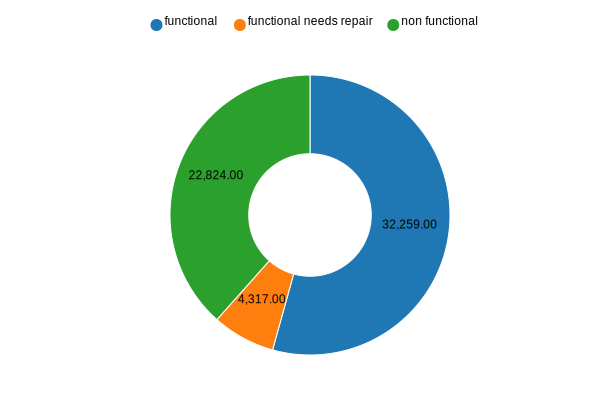
\includegraphics[width=0.5\textwidth]{chart1}
    \caption{Número de instancias de cada clase}
    \label{fig:clases1}
\end{figure}

Las clases están desbalanceadas, observamos una gran diferencia en el número de ejemplos de bombas funcionales y aquellas que pese a ser funcionales requieren mantenimiento. En la Figura \ref{fig:clases2} podemos ver que más de la mitad de las instancias son bombas de agua funcionales (un 54\% de ellas), las no funcionales ocupan un 38\% de las instancias y las funcionales que necesitan reparación forman la clase minoritaria, con tan solo un 7\% de los ejemplos.

\begin{figure}[H]
    \centering
    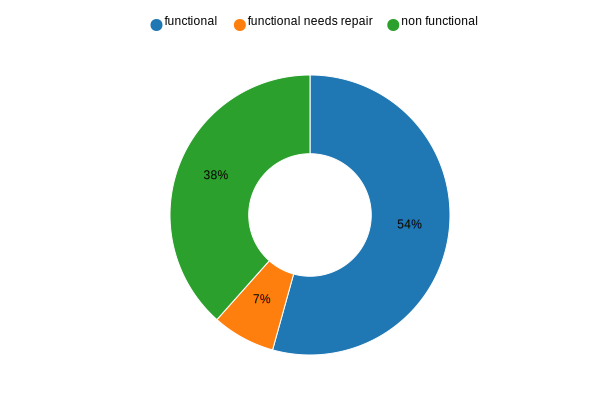
\includegraphics[width=0.5\textwidth]{chart2}
    \caption{Porcentaje de instancias de cada clase}
    \label{fig:clases2}
\end{figure}

Consideraremos como clase positiva ``non functional'', ya que queremos predecir cuáles son las bombas que no funcionan para poder sustituirlas.

Nada más cargar el fichero observamos que es un conjunto de datos que posee valores perdidos, además de algunos valores ``unknown''. 

Toda la experimentación se realizará usando una validación cruzada de 5 particiones. La semilla aleatoria empleada en aquellos algoritmos que lo requieran será: 12345.
Los experimentos realizados en esta práctica se ejecutaron en un ordenador con sistema operativo Ubuntu 16.04 con procesador Intel(R) Core(TM) i5-2410M CPU @ 2.30GHz.

Se utilizará la validación cruzada en la ejecución de todos los algoritmos, mediante los nodos \texttt{X-Partitioner} y \texttt{X-Aggregator} de KNIME. Se configuran para crear 5 particiones, luego en cada experimento se utilizará un conjunto de entrenamiento de tamaño 47520 y un conjunto de prueba formado por 11880 instancias.

Hemos visto en clase que comparar los algoritmos solo por la precisión que consiguen en la predicción no es suficiente, ya que en conjuntos desbalanceados malos algoritmos podrían obtener una alta precisión. Así, utilizaremos medidas sensibles al desbalanceo. Se siguió el tutorial proporcionado por el profesor de prácticas sobre cómo comparar diferentes algoritmos para obtener las tablas de resultados.
%%%%%%%%%%%%%%%%%%%%%%%%%%%%%%%%%%%%%%%%%%%%%%%%%%%%%%%%%%%%%%%%%%%
%       EXPERIMENTOS Y ANÁLISIS DE RESULTADOS
%%%%%%%%%%%%%%%%%%%%%%%%%%%%%%%%%%%%%%%%%%%%%%%%%%%%%%%%%%%%%%%%%%%
\section{Resultados obtenidos}
%%%%%%%%%%%%%%%%%%%%%%%%%%%%%%%%%%%%%%%%%
%%%%%%%       ZeroR
%%%%%%%%%%%%%%%%%%%%%%%%%%%%%%%%%%%%%%%%%
\subsection{ZeroR}
Para comenzar (y sin incluirlo como algoritmo a estudiar), he decidido observar el comportamiento del clasificador ZeroR. Este clasificador predice que cualquier instancia pertenecerá a la clase mayoritaria. Aunque ya sabemos que no obtendremos un buen resultado utilizando este clasificador porque solo clasificará correctamente las instancias que verdaderamente pertenezcan a la clase mayoritaria, nos servirá para tener una cota inferior de las medidas. Si en algún momento durante el desarrollo de la práctica obtuvieramos resultados peores que los obtenidos con este clasificador sospecharemos que estamos haciendo algo mal.

Podemos observar el metanodo creado en KNIME para este algoritmo en la Figura \ref{fig:zeroR}. Se ha utilizado el nodo \texttt{ZeroR} de \texttt{Weka}.

\begin{figure}[H]
    \centering
    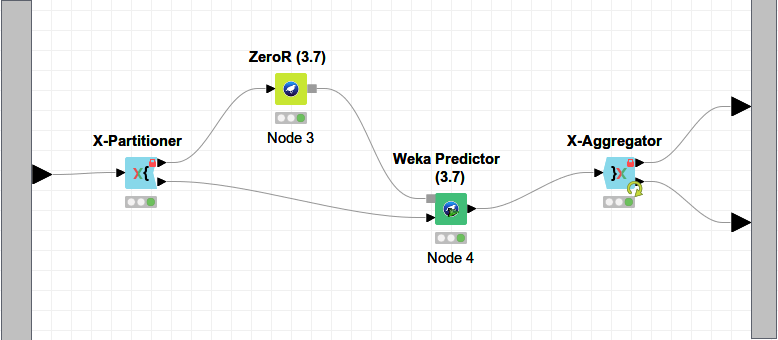
\includegraphics[width=1\textwidth]{ZeroR}
    \caption{Metanodo ZeroR}
    \label{fig:zeroR}
\end{figure}

Utilizamos un nodo \texttt{Scorer} para conocer su matriz de confusión, que encontramos en la Tabla \ref{tab:CMZeroR}, y, tal como debería, todas las instancias son clasificadas como funcionales.

\begin{table}[H]
  \centering
  \caption{ZeroR - Matriz de confusión}
  \label{tab:CMZeroR}
  \begin{tabular}{lrrr}
    \toprule
    & functional & non functional & functional needs repair\\ \midrule
    functional & 32259 & 0 & 0\\
    non functional & 22824 & 0 & 0\\
    functional needs repair & 4317 & 0 & 0\\
    \bottomrule
  \end{tabular}
\end{table}

En la Tabla \ref{tab:zeroR} se encuentran las medidas de precisión obtenidas con este algoritmo. En este caso, conociendo la distribución de las clases, se podrían haber calculado manualmente sin necesidad de ejecutar el algoritmo. Sabemos que todas las instancias serán clasificadas como funcionales y nuestra clase positiva es no funcional, luego no habrá verdaderos positivos (tampoco falsos positivos).

\begin{table}[H]
\centering
\caption{Criterios de precisión}
\label{tab:zeroR}
\begin{tabular}{lrrrrrrrrrrr}
\toprule
row ID & TP & FP & TN & FN & TPR & TNR & PPV & Accur. & F1-score & G-mean & AUC\\ \midrule
ZeroR & 0 & 0 & 36576 & 22824 & 0.0 & 1.0 & ? & 0.6158 & ? & 0.0 & 0.5\\
\bottomrule
\end{tabular}
\end{table}

Nos llaman la atención los datos desconocidos. El PPV, predicciones positivas correctas entre el número total de predicciones positivas es una indeterminación, ya que el número de predicciones positivas (TP) es 0 y el total de predicciones positivas (TP + FP) también lo es. Como el F1-score es la media armónica de PPV y TPR, al no poder calcular el PPV, tampoco podremos calcular el F1-score

%%%%%%%%%%%%%%%%%%%%%%%%%%%%%%%%%%%%%%%%%%%%%%%%%%%%%%%%%%%%%%%%%%%%%
%%%%%%%      CART
%%%%%%%%%%%%%%%%%%%%%%%%%%%%%%%%%%%%%%%%%%%%%%%%%%%%%%%%%%%%%%%%%%%%%

\subsection{Árbol de decisión}

El primer algoritmo elegido es uno basado en árboles de decisión. Estos algoritmos parten de todos los ejemplos y van seleccionando atributos para dividir el conjunto de ejemplos en función al valor de los mismos. Como criterio para seleccionar las variables se utilizará el índice Gini, así que nos encontramos con un algoritmo CART.

El índice Gini mide con qué frecuencia un elemento elegido de forma aleatoria de un conjunto sería etiquetado incorrectamente si se etiqueta aleatoriamente de acuerdo a la distribución de clases en el subconjunto. Dado un conjunto de datos $T$ con ejemplos pertenecientes a $n$ clases, el índice de Gini se define como:
\[gini(T) = 1 - \sum_{j=1}^np_j^2,\] donde $p_j$ es la frecuencia relativa de la clase $j$ en $T$. Este índice valdrá 0 cuando todos los ejemplos de un nodo sean de la misma clase.

Lo ejecutaremos en KNIME mediante ... %TODO

Obtenemos la matriz de confusión mostrada en la Tabla \ref{tab:CMTree}.

\begin{table}[H]
  \centering
  \caption{CART - Matriz de confusión}
  \label{tab:CMTree}
  \begin{tabular}{lrrr}
    \toprule
    & functional & non functional & functional needs repair\\ \midrule
    functional & 26399 & 4265 & 1351\\
    non functional & 4644 & 17456 & 514\\
    funcional needs repair & 2075 & 751 & 1451\\
    \bottomrule
  \end{tabular}
\end{table}

Hemos acudido al nodo \texttt{Scorer} para obtener esta matriz y nos damos cuenta de que tiene un triángulo a modo de advertencia: ``Hay valores perdidos en la referencia o en la predicción de la clase''. Comprobamos que, efectivamente, si sumamos todos los atributos de la matriz de confusión no obtenemos el número total de atributos.
\[26399 + 4265 + 1351 + 4644 + 17456 + 514 + 2075 + 751 + 1451 = 58906 \neq 59400
\]

¿A qué se debe esto? Ya sabemos que el conjunto de datos posee bastantes valores perdidos, estos no causarán problema a la hora de crear el modelo porque cuando nos encontremos con un valor perdido y tengamos que decidir cómo clasificarlo, lo haremos usando la última clase conocida. Es posible que alguna de las clases no aparezca en el conjunto de entrenamiento (functional needs repair, por estar menos representada) y, por tanto, cuando nos encontremos con un ejemplo de este tipo al realizar el test, nuestro modelo no pueda clasificarlo. ??? Esto no puede ser por esto, estamos creando las particiones manteniendo la distribución de clases.

Utilizaremos diferentes índices para poder interpretar la matriz de confusión, podemos verlos en la Tabla \ref{tab:Tree}. 

\begin{table}[H]
\centering
\caption{Criterios de precisión}
\label{tab:Tree}
\begin{tabular}{lrrrrrrrrrrr}
\toprule
 & TP & FP & TN & FN & TPR & TNR & PPV & Accur. & F1-score & G-mean & AUC\\ \midrule
CART & 17456 & 5016 & 31276 & 5158 & 0.7719 & 0.8618 & 0.7768 & 0.8273 & 0.7743 & 0.8156 & 0.8384\\
\bottomrule
\end{tabular}
\end{table}

La utilización de este algoritmo no precisó de ningún preprocesamiento, aceptó todos los atributos. Nos preocupamos porque no sabemos qué está pasando con las variables continuas, que los árboles de decisión no manejan bien, pero vemos en la descripción del nodo que los atributos numéricos (continuos) los dividió en dos subconjuntos a partir de su media para poder tratarlos de forma categórica.

Es un algoritmo robusto, como ya se comentó, es capaz de trabajar con valores perdidos.

Este modelo es fácilmente interpretable, dado un nuevo ejemplo podríamos partir del nodo raíz en el árbol obtenido y llegar a la clase con que se etiquetará siguiendo la rama del árbol correspondiente según el valor de cada atributo.

% TODO Conseguir imagen del árbol

% TODO medir sobreaprendizaje

\subsection{k-NN}
A la hora de clasificar nuestra máxima es la semejanza, partiendo de este criterio el algoritmo más sencillo de entender podría ser el k-NN que realizará la predicción de una instancia en función a sus k vecinos más cercanos. El cálculo de la cercanía se hará en función a la distancia de los distintos atributos, por ello hay que discretizar y normalizar los datos. No podemos trabajar con variables categóricas, ya que no sabríamos medir la distancia euclídea de una palabra a otra. Tampoco podemos trabajar con los datos sin normalizar porque daríamos más importancia a los atributos que tomaran mayores valores.

Comenzamos numerizando las variables. Para ello, utilizamos el nodo \texttt{Category to Number} que dada un atributo con $n$ posibles categorías, asignará un número de 0 hasta $n-1$ a cada categoría. Excluimos la categoría ``class'', pues es la etiqueta que estamos tratando de asignar, aumentamos el número máximo de categorías (el que viene por defecto no sirve para nuestros datos).

A continuación, normalizamos las variables mediante el nodo \texttt{Normalizer}. Ambas operaciones las realizamos antes de la validación cruzada, para el conjunto total de instancias, si normalizaramos solo en el conjunto de entrenamiento, podríamos encontrarnos con valores fuera del rango al realizar el test. Antes de llamar al algoritmo, tenemos que tratar los valores perdidos, en caso contrario, ignorará aquellas filas que los contengan y tendremos problemas en la predicción. Aplicando el nodo \texttt{Missing Value} asignando a los valores numéricos su mediana y a los nominales el más frecuente, sobre el conjunto de entrenamiento (para no utilizar información propia del conjunto de prueba al realizar el modelo). Sobre el conjunto de test aplicamos el nodo \texttt{Missing Value (Apply)}, para que trate los valores perdidos de la forma que se hiciera sobre el conjunto de entrenamiento. Utilizamos el nodo \texttt{K Nearest Neighbor}, que contiene el algoritmo knn tomando como número de vecinos $k = 3$. Además, añadimos un \texttt{Column Rename} para que la columna con la predicción se llame ``Prediction (class)'', como en nuestros otros nodos, en vez de ``Class [kNN]''. El flujo en KNIME es el mostrado en la Figura \ref{fig:3nn}.

\begin{figure}[H]
    \centering
    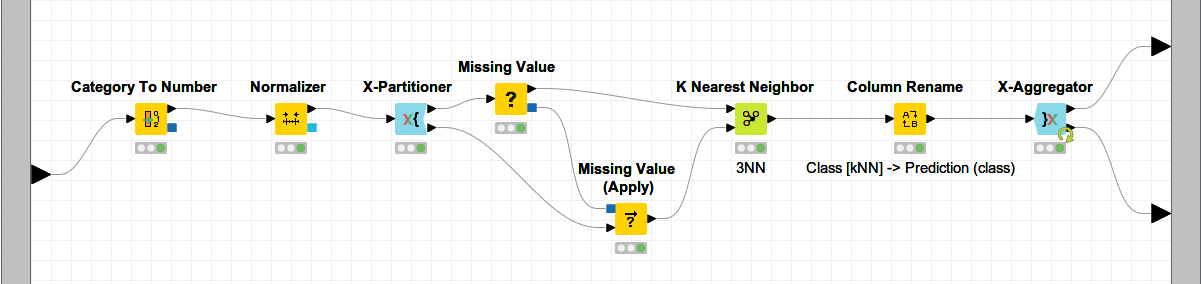
\includegraphics[width=1\textwidth]{3nn}
    \caption{Metanodo 3-NN}
    \label{fig:3nn}
\end{figure}.

A continuación, en la Tabla \ref{tab:CM3nn}, se muestra la matriz de confusión para este algoritmo.

\begin{table}[H]
\centering
\caption{3-NN - Matriz de confusión}
\label{tab:CM3nn}
\begin{tabular}{lrrr}
\toprule
row ID & functional & non functional & functional needs repair\\ \midrule
functional & 26884 & 4378 & 997\\
non functional & 6410 & 15925 & 489\\
functional needs repair & 2412 & 747 & 1158\\
\bottomrule
\end{tabular}
\end{table}

%% Comprobamos el número de instancias clasificadas y vemos que, como venía advirtiendo el nodo \texttt{K Nearest Neighbor}, es bastante inferior al número de instancias:
%% 26884+4378+997+6410+2412+747+1158 = 42986
% \neq 59400.
%% \]

En la Tabla \ref{tab:3nn} se muestran los diferentes criterios de precisión para este algoritmo.

\begin{table}[H]
\centering
\caption{3-NN - Criterios de precisión}
\label{tab:3nn}
\begin{tabular}{lrrrrrrrrrrr}
\toprule
 & TP & FP & TN & FN & TPR & TNR & PPV & Accur. & F1-score & G-mean & AUC\\ \midrule
3NN & 15925 & 5125 & 31451 & 6899 & 0.6977 & 0.8599 & 0.7565 & 0.7976 & 0.7259 & 0.7746 & 0.8408\\
\bottomrule
\end{tabular}
\end{table}
%%%%%%%%%%%%%%%%%%%%%%%%%%%%%%%%%%%%%%%%%%%%%%%%%%%%%%%%%%%%%%%%%%
%               RED NEURONAL - MLP
%%%%%%%%%%%%%%%%%%%%%%%%%%%%%%%%%%%%%%%%%%%%%%%%%%%%%%%%%%%%%%%%%%
\subsection{Red neuronal}

Se ha escogido una red neuronal como siguiente algoritmo. Los algoritmos de redes neuronales se inspiran en las redes neuronales biológicas. Tienen unos nodos (llamados neuronas) que se conectan con otros nodos, transmitiendo una señal que será un número real. Estas conexiones tienen un peso que se va ajustando en el proceso de aprendizaje.  

En este caso también es necesario que los valores sean numéricos y estén normalizados. Además, aunque el nodo \texttt{Learner} permita ignorar los valores perdidos, si estos llegan al nodo \texttt{Predictor} obtendremos un error, luego es necesario manejarlos en nuestro preprocesamiento mínimo del algoritmo.

Comenzamos transformando a número los datos categóricos mediante el nodo \texttt{Category to Number}. Seguidamente, los normalizamos usando el nodo \texttt{Normalize} y mediante los nodos \texttt{X-Partitioner}, \texttt{X-Aggregator} realizaremos la validación cruzada. Tenemos que tratar los valores perdidos, para ello utilizamos el nodo \texttt{Missing Value} en la rama de entrenamiento y sustituimos los valores numéricos perdidos por su mediana y los categóricos por el más frecuente. En la rama de test usamos el nodo \texttt{Missing Value (Apply)} que aplicará las transformaciones del nodo \texttt{Missing Value}. Así, el metanodo en KNIME correspondiente al modelado de la red neuronal queda como se ve en la Figura \ref{fig:MLP}. 

\begin{figure}[H]
    \centering
    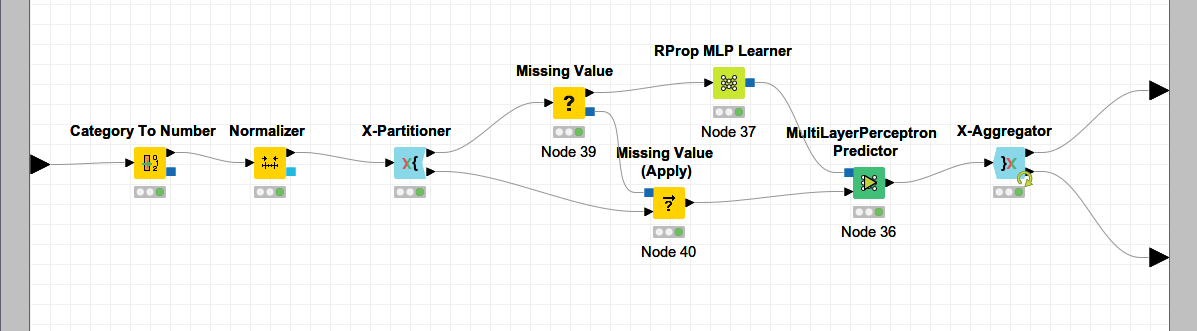
\includegraphics[width=1\textwidth]{MLP}
    \caption{Metanodo MLP}
    \label{fig:MLP}
\end{figure}

Se utilizan los nodos \texttt{RProp MLP Learner} y \texttt{MultiLayerPerceptron Predictor} para modelar y probar este algoritmo. La red neuronal realizará un máximo de 100 iteraciones, tendrá una única capa oculta con 10 neuronas por capa.

La matriz de confusión obtenida la encontramos en la Tabla \ref{tab:CMMLP}.

\begin{table}[H]
\centering
\caption{Red Neuronal - Matriz de confusión}
\label{tab:CMMLP}
\begin{tabular}{lrrr}
\toprule
 & functional & non functional & functional needs repair\\ \midrule
functional & 27361 & 4873 & 25\\
non functional & 9183 & 13620 & 21\\
functional needs repair & 3359 & 900 & 58\\
\bottomrule
\end{tabular}
\end{table}


Las diferentes medidas de precisión asociadas a este algoritmo las vemos en la Tabla \ref{tab:MLP}.

\begin{table}[H]
\centering
\caption{Red Neuronal - Criterios de precisión}
\label{tab:MLP}
\begin{tabular}{lrrrrrrrrrrr}
\toprule
 & TP & FP & TN & FN & TPR & TNR & PPV & Accur. & F1-score & G-mean & AUC\\ \midrule
MLP & 13777 & 6090 & 30486 & 9047 & 0.6036 & 0.8335 & 0.6935 & 0.7452 & 0.6454 & 0.7093 & 0.7934\\
\bottomrule
\end{tabular}
\end{table}


\subsection{Naive Bayes}

El siguiente algoritmo elegido es uno basado en métodos bayesianos. Asume que los atributos son independientes y calcula la clase más probable condicionando el valor del resto de atributos.

Lo utilizamos en nuestra validación cruzada mediante los nodos \texttt{Naive Bayes Learner} y \texttt{Naive Bayes Predictor}, que dejamos con sus valores por defecto. El metanodo Naive Bayes creado en KNIME para este algoritmo se presenta en la Figura \ref{fig:NaiveBayes}.

\begin{figure}[H]
    \centering
    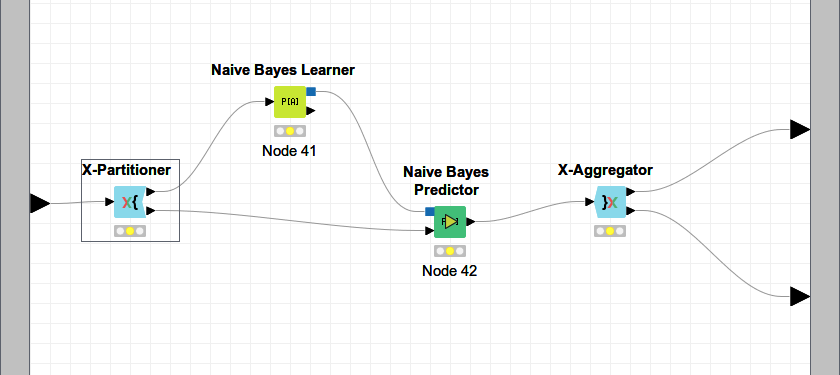
\includegraphics[width=1\textwidth]{NaiveBayes}
    \caption{Metanodo Naive Bayes}
    \label{fig:NaiveBayes}
\end{figure}

Notamos que este algoritmo no necesita ningún preprocesamiento mínimo, trabaja tanto con variables numéricas como con variables categóricas, no es necesario que las normalicemos y aunque obtenemos una advertencia de que hay valores perdidos es capaz de obtener información sobre ellos que luego usará en el predictor.

La matriz de confusión obtenida mediante el uso de este algoritmo la podemos encontrar en la Tabla \ref{tab:CMNaiveBayes}.

\begin{table}[H]
\centering
  \caption{Naive Bayes - Matriz de confusión}
  \label{tab:CMNaiveBayes}
  \begin{tabular}{lrrr}
\toprule
    & functional & non functional & functional needs repair\\ \midrule
    functional & 18426 & 7036 & 6797\\
    non functional & 3699 & 16087 & 3038\\
    functional needs repair & 648 & 800 & 2869\\
    \bottomrule
  \end{tabular}
\end{table}

Las diferentes medidas de precisión aparecen en la Tabla \ref{tab:NaiveBayes}.
\begin{table}[H]
\centering
\caption{Naive Bayes - Criterios de precisión}
\label{tab:NaiveBayes}
\begin{tabular}{lrrrrrrrrrrr}
\toprule
 & TP & FP & TN & FN & TPR & TNR & PPV & Accur. & F1-score & G-mean & AUC\\ \midrule
NB & 16087 & 7836 & 28740 & 6737 & 0.7048 & 0.7858 & 0.6724 & 0.7547 & 0.6883 & 0.7442 & 0.8258\\
\bottomrule
\end{tabular}
\end{table}
\subsection{Random Forest}

Pasamos ahora a un multiclasificador que combina varios clasificadores simples para tratar de mejorar la clasificación. Este primer multiclasificador será un ejemplo de \textit{bagging}, esto es cada clasificador se induce independientemente sin información de los demás. Busca mejorar algoritmos inestables, que frente a pequeños cambios en el conjunto de entrenamiento pueden provocar grandes cambios en la predicción.

Se ha escogido el algoritmo Random Forest, que realiza distintas clasificaciones con árboles más débiles (que no consideran todas las variables, sin poda) y con diferentes subconjuntos de los datos. Para realizar el modelo utilizaremos el nodo \texttt{Random Forest Learner}, que es probado mediante el nodo \texttt{Random Forest Predictor}. 

El flujo en KNIME es el que vemos en la Figura \ref{fig:RandomForest} y los nodos han sido configurados para utilizar 100 clasificadores que utilicen el índice Gini para elegir los atributos por los que ramificar el árbol. Ha sido necesario usar el nodo \texttt{Domain Calculator}, sin restringir el número de posibles valores, para que tuviera en cuenta todas las variables.

\begin{figure}[H]
    \centering
    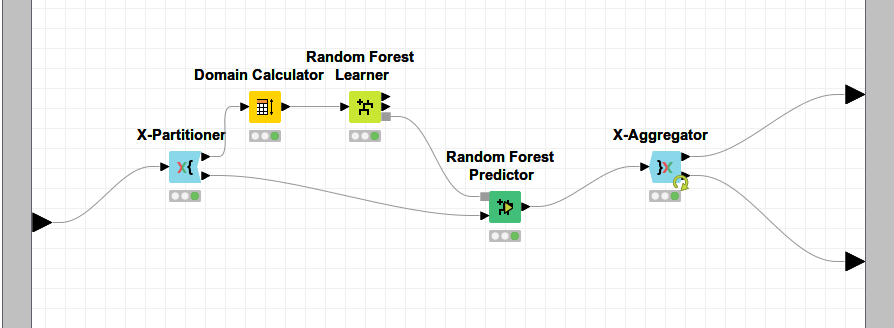
\includegraphics[width=1\textwidth]{RandomForest}
    \caption{Metanodo Random Forest}
    \label{fig:RandomForest}
\end{figure}

En la Tabla \ref{tab:RandomForest} observamos la matriz de confusión obtenida mediante el uso de este algoritmo.

\begin{table}[H]
\centering
\caption{-Matriz de confusión}
\label{tab:CMRandomForest}
\begin{tabular}{lrrrr}
\toprule
 & functional & non functional & functional needs repair\\ \midrule
functional & 29630 & 2126 & 503\\
non functional & 5224 & 17341 & 259\\
functional needs repair & 2484 & 548 & 1285\\
\bottomrule
\end{tabular}
\end{table}

En la Tabla \ref{tab:RandomForest} se encuentran las medidas de precisión conseguidas por este algoritmo.

\begin{table}[H]
\centering
\caption{Random Forest - Criterios de precisión}
\label{tab:RandomForest}
\begin{tabular}{lrrrrrrrrrrr}
\toprule
 & TP & FP & TN & FN & TPR & TNR & PPV & Accur. & F1-score & G-mean & AUC\\ \midrule
RF & 17341 & 2674 & 33902 & 5483 & 0.7598 & 0.9269 & 0.8664 & 0.8627 & 0.8096 & 0.8392 & 0.9243\\
\bottomrule
\end{tabular}
\end{table}


Al ser un algoritmo que combina muchos árboles y estos admitir valores perdidos, Random Forest también admitirá valores perdidos. Sin embargo, la interpretabilidad de este modelo no es tan alta como lo era la de un único árbol de decisión. En el análisis compararemos los resultados de este algoritmo frente a un único árbol de decisión.

% TODO medir complejidad

\subsection{Boosting}

Probamos en este caso un algoritmo de \textit{boosting}, esto es, un multiclasificador en el que cada clasificador tiene en cuenta los fallos del anterior.

Elegimos el nodo \texttt{XGBoosting Tree Ensemble Learner}, para realizar un modelo basado en árboles. Es necesario que numericemos las variables para no encontrarnos con problemas al predecir, así que añadimos el nodo \texttt{Category To Number} antes de realizar la partición. Vemos en la Figura \ref{fig:XGBoost} cómo quedó el flujo en KNIME necesario para ejecutar un algoritmo de \textit{boosting}.

\begin{figure}[H]
    \centering
    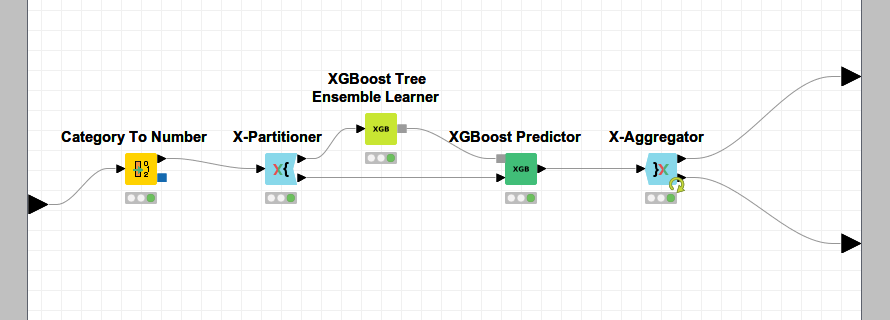
\includegraphics[width=1\textwidth]{XGBoost}
    \caption{Metanodo XGBoost}
    \label{fig:XGBoost}
\end{figure}

Las tasas de clasificación obtenidas con este algoritmo las podemos visualizar en la Tabla \ref{tab:CMXGB}.

\begin{table}[H]
  \centering
  \caption{XGBoost - Matriz de confusión}
  \label{tab:CMXGB} 
  \begin{tabular}{lrrr}
    \toprule
    row ID & functional & non functional & functional needs repair\\ \midrule
    functional & 29290 & 2533 & 436\\
    non functional & 5438 & 17140 & 246\\
    functional needs repair & 2506 & 624 & 1187\\
    \bottomrule
  \end{tabular}
\end{table}

Notamos que, aunque este algoritmo ha necesitado un mínimo preprocesado para admitir todas las variables del conjunto de datos, no fue necesario rellenar los valores perdidos. Comprobamos en \ref{ref:XGB} que este algoritmo soporta por defecto los valores peridos, durante el entrenamiento se trata con ellos.

Las medidas de precisión obtenidas para este algoritmo son las detalladas en la Tabla \ref{tab:XGB}.

\begin{table}[H]
\centering
\caption{XGBoost - Criterios de precisión}
\label{tab:XGB}
\begin{tabular}{lrrrrrrrrrrr}
\toprule
 & TP & FP & TN & FN & TPR & TNR & PPV & Accur. & F1-score & G-mean & AUC\\ \midrule
XGB & 17140 & 3157 & 33419 & 5684 & 0.751 & 0.9137 & 0.8445 & 0.8512 & 0.795 & 0.8283 & 0.9182\\
\bottomrule
\end{tabular}
\end{table}
%%%%%%%%%%%%%%%%%%%%%%%%%%%%%%%%%%%%%%%%%%%%%%%%%%%%%%%%%%%%%%%%%%%%%
%%%%%%% ANÁLISIS DE RESULTADOS
%%%%%%%%%%%%%%%%%%%%%%%%%%%%%%%%%%%%%%%%%%%%%%%%%%%%%%%%%%%%%%%%%%%%%
\section{Análisis de resultados}

Al ver los datos de cada uno de los algoritmos de forma independiente, pocas conclusiones podemos extraer. No conocemos unos umbrales generales (más allá de los que pueda aportar un clasificador aleatorio o el ZeroR) que nos permitan determinar si un algoritmo es o no bueno. ¿Cómo comparamos el rendimiento de los algoritmos? ¿Nos centramos en su precisión e imponemos un umbral? Imponer un umbral no es posible, para cada conjunto de datos los resultados de los algoritmos varían mucho. Además, atender solo a la precisión nos puede llevar a conclusiones erróneas, especialmente cuando estamos ante un conjunto de clases desbalanceadas.

Por ello, realizaremos un análisis comparativo, centrado en las diferencias entre los algoritmos y en sus causas. En la Tabla \ref{tab:global} se recogen los criterios de precisión obtenidos con los algoritmos elegidos.

\begin{table}[H]
\centering
\caption{Criterios de precisión}
\label{tab:global}
\begin{tabular}{lrrrrrrrrrrr}
\toprule
 & TP & FP & TN & FN & TPR & TNR & PPV & Accur. & F1-score & G-mean & AUC\\ \midrule
ZeroR & 0 & 0 & 36576 & 22824 & 0.0 & 1.0 & ? & 0.6158 & ? & 0.0 & 0.5\\
CART & 17456 & 5016 & 31276 & 5158 & 0.7719 & 0.8618 & 0.7768 & 0.8273 & 0.7743 & 0.8156 & 0.8384\\
3NN & 15925 & 5125 & 31451 & 6899 & 0.6977 & 0.8599 & 0.7565 & 0.7976 & 0.7259 & 0.7746 & 0.8408\\
MLP & 13777 & 6090 & 30486 & 9047 & 0.6036 & 0.8335 & 0.6935 & 0.7452 & 0.6454 & 0.7093 & 0.7934\\
NB & 16087 & 7836 & 28740 & 6737 & 0.7048 & 0.7858 & 0.6724 & 0.7547 & 0.6883 & 0.7442 & 0.8258\\
RF & 17341 & 2674 & 33902 & 5483 & 0.7598 & 0.9269 & 0.8664 & 0.8627 & 0.8096 & 0.8392 & 0.9243\\
XGB & 17140 & 3157 & 33419 & 5684 & 0.751 & 0.9137 & 0.8445 & 0.8512 & 0.795 & 0.8283 & 0.9182\\
\bottomrule
\end{tabular}
\end{table}

% TP, FP, TN, FN
Comenzamos atendiendo a las matrices de confusión de los diferentes algoritmos. En la Figura \ref{fig:CM} podemos observar las tasas de acierto y fallo de los algoritmos considerados, teniendo en cuenta que nuestra clase positiva es ``no funcional''.

\begin{figure}[H]
    \centering
    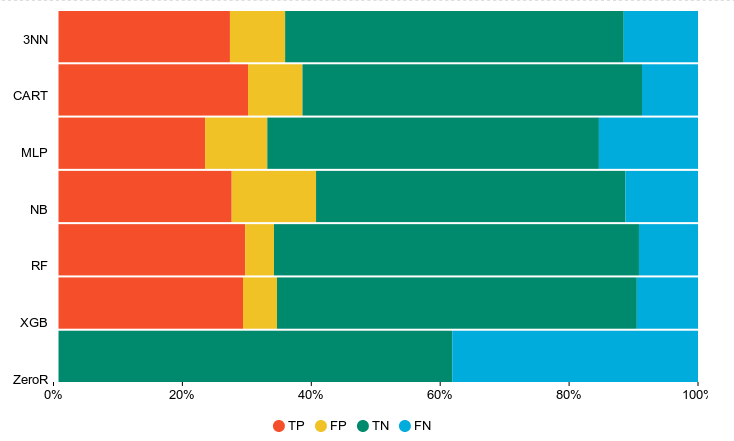
\includegraphics[width=1\textwidth]{CM}
    \caption{Tasas de acierto y error}
    \label{fig:CM}
\end{figure}

Buscamos aquellos algoritmos que sean capaces de predecir correctamente las bombas de agua que no funcionan, esto es, que el número de verdaderos positivos (TP) sea lo más grande posible. Los algoritmos que mejor consiguen esto son CART, RandomForest y XGBoost, todos los basados en árboles. Por otro lado, nos interesa que bombas no funcionales no sean clasificadas como sí funcionales, es decir, que los falsos negativos sean los menos posibles (FN). Vuelven a conseguir mejores resultados los algoritmos basados en árboles. Es posible que esto se deba a que los algoritmos basados en árboles trabajan bien tanto con variables numéricas como categóricas y no precisaron numerizar las variables nominales (con las desventajes que esto puede traer).

% ACCURACY
Pasamos a comparar la precisión de los distintos algoritmos, para visualizar mejor este dato se ha utilizado el gráfico de barras mostrado en la Figura \ref{fig:accuracy}

\begin{figure}[H]
    \centering
    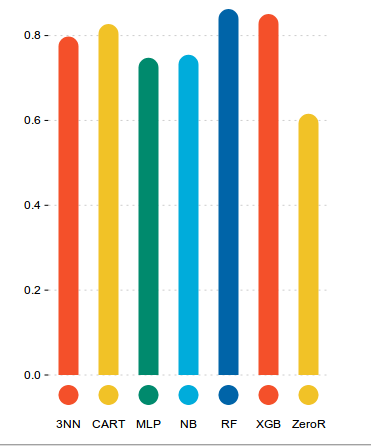
\includegraphics[width=0.5\textwidth]{Accuracy}
    \caption{Precisión de los distintos algoritmos}
    \label{fig:accuracy}
\end{figure}

Destacamos que solo superan el umbral de 0.8 los tres algoritmos basados en árboles de decisión, quedando por encima los multiclasificadores y seguidos muy de cerca por el 3-NN. Aunque a todos los algoritmos les favorezca el preprocesado de los datos, ya que se eliminan algunos problemas proveniente de ellos o se les da una solución razonable, son los algoritmos basados en árboles los que mejor trabajan con los datos en sí mismos. No requieren ningún preprocesado, que sí que requiere el 3-NN, por ejemplo. El preprocesado mínimo y poco exhaustivo puede ser la razón de que la precisión del 3-NN no supere la de los árboles de decisión.

Las redes neuronales son muy difíciles de ajustar y era bastante complicado que la configuración por defecto fuera la apropiada para nuestro problema. En Naive Bayes estamos haciendo una suposición que comprobaremos que no se cumple, no todas las variables son independientes.

% Curva ROC
Sabemos que en los problemas complejos, como es el nuestro, aumentar el número de aciertos en la clase positiva, se hace a costa de incrementar también el número de errores en dicha clase. Buscamos un clasificador que aumente los verdaderos positivos a un ritmo mayor que al que aumenta el de falsos positivos. Para encontrarlos o detectarlos utilizamos la curva ROC y el índice AUC (Area Under the Curve), cuando más se acerque a 1 este índice, más no acercaremos al clasificador buscado. En la Figura \ref{fig:ROC} podemos observar la curva ROC de los algoritmos ejecutados y, al lado del nombre de cada algoritmo entre paréntesis, el área bajo la curva.

\begin{figure}[H]
    \centering
    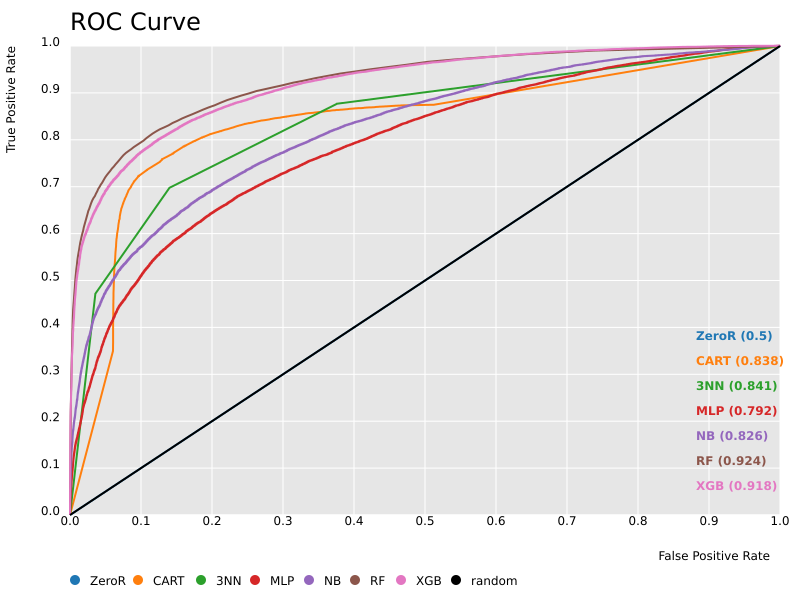
\includegraphics[width=1\textwidth]{ROC}
    \caption{Curva ROC}
    \label{fig:ROC}
\end{figure}

En primer lugar, notamos que la curva ROC del algoritmo ZeroR coincide con la de un clasificador aleatorio, no supone ninguna diferencia en este aspecto etiquetar aleatoriamente los elementos o etiquetarlos todos de la misma forma.

Los algoritmos que consiguen mayor valor AUC son RandomForest y XGBoost, aquí observamos la potencia que añaden los multiclasificadores sobre los clasificadores simples. Aprovechando los resultados no demasiado malos que conseguimos con los árboles de decisión (CART - 0.838 AUC) logran superarlos casi por una decena al combinar muchos de ellos.

El algoritmo que peor índice AUC obtiene es la red neuronal, tendremos que probar a adaptar sus parámetros para conseguir mejores resultados para este conjunto de datos.

El 3-NN supera al algoritmo CART en área bajo la curva. %TODO POR QUÉ

Naive Bayes supera a la red neuronal probada, pero mantiene una tasa menor que el resto de algoritmos. Esto se puede deber a que asume que las variables son independientes y en función a ello crea el modelo. Tendremos que comprobar que eliminando las variables dependientes mejora su resultado. % TODO COMPROBAR ESO

% TODO estudiar sobreaprendizaje de CART, RF, XGB Y 3NN, comentar

%%%%%%%%%%%%%%%%%%%%%%%%%%%%%%%%%%%%%%%%%%%%%%%%%%%%%%%%%%%%%%%%%%%
%%% CONFIGURACIÓN DE ALGORITMOS
%%%%%%%%%%%%%%%%%%%%%%%%%%%%%%%%%%%%%%%%%%%%%%%%%%%%%%%%%%%%%%%%%%
\section{Configuración de algoritmos}

En esta sección se configurarán los distintos parámetros de algunos algoritmos. Por un lado, trataremos de que aquellos algoritmos con peores resultados para los índices estudiados consigan alcanzar a los que consiguieron mejores resultados. Por otro, trataremos de que los algoritmos que superaron al resto, lleguen a mayores valores de estos índices.

\subsection{k-NN}

Comenzamos estudiando el comportamiento del k-NN al aumentar el valor de k, esto es, el número de vecinos cercanos que se utiliza para clasificar. Copiaremos el metanodo anterior y solo modificaremos el número de vecinos, probaremos con 5, con 7 y con 1. En la Tabla \ref{tab:knn} se muestran las medidas de precisión obtenidas para el algoritmo con las 4 opciones consideradas para el parámetro k. A priori no podemos saber si aumentar o disminuir este valor supondrá o no una mejora para este conjunto de datos. No  existe un k genérico que funcione bien con todo tipo de problemas, así a base de pruebas determinaremos cuál funciona mejor para nuestro conjunto de datos.

\begin{table}[H]
\centering
\caption{k-NN - Criterios de precisión}
\label{tab:}
\begin{tabular}{lrrrrrrrrrrr}
\toprule
 & TP & FP & TN & FN & TPR & TNR & PPV & Accur. & F1-score & G-mean & AUC\\ \midrule
1NN & 16331 & 6097 & 30479 & 6493 & 0.7155 & 0.8333 & 0.7282 & 0.788 & 0.7218 & 0.7722 & 0.7745\\
3NN & 15925 & 5125 & 31451 & 6899 & 0.6977 & 0.8599 & 0.7565 & 0.7976 & 0.7259 & 0.7746 & 0.8408\\
5NN & 15723 & 5192 & 31384 & 7101 & 0.6889 & 0.858 & 0.7518 & 0.793 & 0.7189 & 0.7688 & 0.8516\\
7NN & 15518 & 5125 & 31451 & 7306 & 0.6799 & 0.8599 & 0.7517 & 0.7907 & 0.714 & 0.7646 & 0.8562\\
\bottomrule
\end{tabular}
\end{table}

Vemos que el 1-NN, pese a ser el que más aciertos sobre la clase positiva tiene, es el que peores índices de precisión tiene (excepto el TPR), pues aumenta la clasificación de positivos y con ello tanto los verdaderos positivos, como los falsos positivos. Este hecho se ve reflejado en su valor AUC, notablemente menor que para el resto de valores de k. 
Observamos que, a medida que aumentamos el número de vecinos a considerar, las medidas de presición disminuyen todas excepto el área bajo la curva ROC. Un motivo por el que puede resultar perjudicial aumentar el número de vecinos es que los elementos que se encuentren en la frontera entre dos clases, más cerca de la clase contraria, pueden verse etiquetados como elemento de la clase contraria al utilizar más vecinos para su clasificación.

Así, nos quedamos con el valor k que habíamos escogido inicialmente, k = 3.

Procedemos ahora con una segunda modificación sobre el 3-NN. Añadiremos un peso a los vecinos, los más cercanos tendrán un peso mayor que los más lejanos. Este cambio pretende clasificar mejor aquellas instancias que se encuentren alejadas de sus clases. En la Tabla \ref{tab:knnwd} observamos los criterios de precisión asociados y los comparamos con el 3-NN sin modificar.

\begin{table}[H]
\centering
\caption{3-NN - Criterios de precisión}
\label{tab:knnwd}
\begin{tabular}{lrrrrrrrrrrr}
\toprule
 & TP & FP & TN & FN & TPR & TNR & PPV & Accur. & F1-score & G-mean & AUC\\ \midrule
3NN & 15925 & 5125 & 31451 & 6899 & 0.6977 & 0.8599 & 0.7565 & 0.7976 & 0.7259 & 0.7746 & 0.8408\\
3NN-wd & 16373 & 5565 & 31011 & 6451 & 0.7174 & 0.8479 & 0.7463 & 0.7977 & 0.7316 & 0.7799 & 0.8475\\
\bottomrule
\end{tabular}
\end{table}

La precisión obtenida por ambos algoritmos es similar, sin embargo, para el resto de valores medios (F1-scores, G-mean) y AUC esta modificación supone una leve mejora. Por ello, nos quedamos con el 3-NN ponderado como clasificador.

Aunque si volvemos a la Tabla \ref{tab:global}, vemos que incluso el mejor k-NN no alcanza a los algoritmos basados en árboles.

\subsection{Red neuronal}

Pasamos ahora a configurar los parámetros de la red neuronal, la configuración por defecto no consiguió buenos resultados, pero esto no significa que el algoritmo no funcione bien. Nos disponemos a modificar algunos parámetros (número de capas y número de neuronas por capa) para ver si obtenemos mejores índices de presición.

En la Tabla \ref{tab:MLPmod} observamos los resultados obtenidos con diferentes configuraciones. Utiliza la expresión MLP \texttt{nºcapas }c \texttt{nº neuronas por capa} nc.

\begin{table}[H]
\centering
\caption{MLP modificada - Criterios de precisión}
\label{tab:MLPmod}
\begin{tabular}{lrrrrrrrrrrr}
\toprule
& TP & FP & TN & FN & TPR & TNR & PPV & Accur. & F1-score & G-mean & AUC\\ \midrule
MLP & 13620 & 5773 & 30803 & 9204 & 0.5967 & 0.8422 & 0.7023 & 0.7479 & 0.6452 & 0.7089 & 0.7917\\
MLP-5c & 13145 & 5750 & 30826 & 9679 & 0.5759 & 0.8428 & 0.6957 & 0.7403 & 0.6302 & 0.6967 & 0.7815\\
MLP-3c25nc & 13544 & 4547 & 32029 & 9280 & 0.5934 & 0.8757 & 0.7487 & 0.7672 & 0.6621 & 0.7209 & 0.8136\\
MLP-5c20nc & 12701 & 3803 & 32773 & 10123 & 0.5565 & 0.896 & 0.7696 & 0.7656 & 0.6459 & 0.7061 & 0.8022\\
MLP-2c5nc & 12937 & 5436 & 31140 & 9887 & 0.5668 & 0.8514 & 0.7041 & 0.742 & 0.6281 & 0.6947 & 0.7789\\
\bottomrule
\end{tabular}
\end{table}

Las variaciones en la arquitectura de la red neuronal no nos proporcionaron grandes mejoras en su rendimiento. Atendiendo a accuracy, F1-score, G-mean y AUC determinamos que la red neuronal formada por 3 capas con 25 neuronas por capa es la mejor que hemos encontrado. Mediante estas pruebas aprendemos que la determinación de la mejor arquitectura de una red neuronal para un problema concreto no es un proceso sencillo y requiere dedicarle mucho tiempo en un proceso de prueba y error.

\subsection{RandomForest}

El algoritmo que mejor medidas nos ha dado es RandomForest, procedemos a modificar sus parámetros a ver si conseguimos mejorar todavía más estos resultados.

En primer lugar, cambiamos el criterio de división del árbol, para que pase a ser ``Info Gain Ratio''.

\begin{table}[H]
\centering
\caption{RandomForest - Criterios de precisión}
\label{tab:rfgainratio}
\begin{tabular}{lrrrrrrrrrrr}
\toprule
 & TP & FP & TN & FN & TPR & TNR & PPV & Accur. & F1-score & G-mean & AUC\\ \midrule
RF & 17341 & 2674 & 33902 & 5483 & 0.7598 & 0.9269 & 0.8664 & 0.8627 & 0.8096 & 0.8392 & 0.9243\\
RF-GR & 11813 & 1849 & 34727 & 11011 & 0.5176 & 0.9494 & 0.8647 & 0.7835 & 0.6475 & 0.701 & 0.857\\
\bottomrule
\end{tabular}
\end{table}

En la Tabla \ref{tab:rfgainratio} observamos que los resultados obtenidos no suponen ninguna mejora, de hecho empeoran los resultados que había obtenido el RandomForest, así que nos quedaremos con el índice Gini para comprobar si con más iteraciones del algoritmo se consiguen mejores resultados. En la Tabla \ref{tab:rf125} se exponen las medidas de presición para RandomForest con 100 y 125 iteraciones.

\begin{table}[H]
\centering
\caption{RandomForest - Criterios de precisión}
\label{tab:rf125}
\begin{tabular}{lrrrrrrrrrrr}
\toprule
 & TP & FP & TN & FN & TPR & TNR & PPV & Accur. & F1-score & G-mean & AUC\\ \midrule
RF & 17341 & 2674 & 33902 & 5483 & 0.7598 & 0.9269 & 0.8664 & 0.8627 & 0.8096 & 0.8392 & 0.9243\\
RF125 & 17374 & 2674 & 33902 & 5450 & 0.7612 & 0.9269 & 0.8666 & 0.8632 & 0.8105 & 0.84 & 0.9247\\
\bottomrule
\end{tabular}
\end{table}

Se observa una ligera mejora al utilizar más árboles en el RandomForest, pero la diferencia es tan pequeña que no compensa el tiempo de cómputo necesario.

\subsection{XGBoost}

En el algoritmo de boosting elegido se puede modificar el número de iteraciones dadas. En la Tabla \ref{tab:xgbmod} encontramos los resultados para 125 y 150 iteraciones.

\begin{table}[H]
\centering
\caption{XGBoost nº iteraciones - Criterios de precisión}
\label{tab:}
\begin{tabular}{lrrrrrrrrrrr}
\toprule
 & TP & FP & TN & FN & TPR & TNR & PPV & Accur. & F1-score & G-mean & AUC\\ \midrule
XGB & 17140 & 3157 & 33419 & 5684 & 0.751 & 0.9137 & 0.8445 & 0.8512 & 0.795 & 0.8283 & 0.9182\\
XGB-125 & 17297 & 3178 & 33398 & 5527 & 0.7578 & 0.9131 & 0.8448 & 0.8535 & 0.799 & 0.8319 & 0.9202\\
XGB-150 & 17405 & 3206 & 33370 & 5419 & 0.7626 & 0.9123 & 0.8445 & 0.8548 & 0.8014 & 0.8341 & 0.9215\\
XGB-250 & 17675 & 3304 & 33272 & 5149 & 0.7744 & 0.9097 & 0.8425 & 0.8577 & 0.807 & 0.8393 & 0.9229\\
\bottomrule
\end{tabular}
\end{table}

Al aumentar el número de iteraciones aumenta el número de aciertos. Esto se debe a que en cada iteración se llama a un algoritmo simple pasándole un conjunto de datos en el que estos están ponderados en función de cómo han sido clasificados anteriormente, así, cuantas más iteraciones realicemos, el clasificador mejor aprenderá a distinguir las instancias más difíciles.

El incremento en el número de verdaderos positivos se crea mediante una disminución del número de falsos negativos, esto es, al aumentar el número de iteraciones etiquetamos menos como funcionales (precisen o no de reparación) a bombas de agua que en realidad no lo eran. La precisión, el F1-score, G-mean y AUC se elevan con el aumento de iteraciones.

\section{Procesado de datos}
\label{Preprocesado}
\section{Interpretación de resultados}

\section{Contenido adicional}
%%%%%%%%%%%%%%%%%%%%%%%%%%%%%%%%%%%%%%%%%%%%%%%%%%%%%%%%%%%%%%%%%%%
%       REFERENCIAS
%%%%%%%%%%%%%%%%%%%%%%%%%%%%%%%%%%%%%%%%%%%%%%%%%%%%%%%%%%%%%%%%%%%
\section{Bibliografía}
% https://en.wikipedia.org/wiki/Decision_tree_learning#Gini_impurity
% https://en.wikipedia.org/wiki/Confusion_matrix
\label{ref:XGB}%https://xgboost.readthedocs.io/en/latest/faq.html
% https://plotdb.com/
\end{document}
